\chapter{Resultados e Discussões}
\label{cap:resultados}

A partir das especificações descritas no capítulo 5, foram implementados todos os componentes que fazem parte da arquitetura proposta para o estudo de caso deste trabalho. Neste capítulo apresentam-se os resultados obtidos após a etapa de desenvolvimento. Na seção \ref{sec:coleta}, são exibidos os resultados encontrados após a etapa de coleta de dados. Na seção \ref{sec:sent-ana}, discute-se a fase de análise de sentimentos das mensagens pesquisadas. Por fim, na seção \ref{sec:proc-web}, são apresentados os resultados do processamento ocorrido no Hive e também da construção da interface \textit{web}.

\section{Coleta de Dados}
\label{sec:coleta}

Durante o processo de busca por postagens provenientes das redes sociais escolhidas como fonte de pesquisa, foram coletados aproximadamente 600MB de arquivos no formato JSON. Estes dados correspondem às mensagens publicadas no período entre janeiro de 2014 e abril de 2015, além de conter outras informações relevantes, como especificado no modelo de dados descrito na figura \ref{tables}. A tabela \ref{tab-result-fb-tw} apresenta a quantidade exata de mensagens obtidas a partir das APIs do Facebook e Twitter, combinadas com a implementação de \textit{souces} do Flume.

\begin{table}[!ht]
\begin{center}
  \begin{tabular}{|p{5cm}|p{5cm}|}
	\hline
	Fonte de dados & Quantidade de mensagens
	\\ \hline
	Facebook & 1612701
	\\ \hline
	Twitter & 113990
	\\ \hline
  \end{tabular}
  \captionsetup{justification=centering}
  \caption[Quantidade de mensagens coletadas]{Quantidade de mensagens coletadas
  \protect\linebreak Fonte: Autor}
\label{tab-result-fb-tw}
\end{center}
\end{table}
\FloatBarrier

A busca pela coleta de uma grande quantidade de mensagens acabou se tornando um dos principais obstáculos encontrados nesta fase do trabalho. As limitações impostas pelas APIs das redes sociais influenciaram diretamente para que o número de publicações obtidas não apresentasse um resultado mais expressivo, quando comparado ao potencial destes meios. O Twitter, como mencionado anteriormente, apenas permite buscas por mensagens recentes, além de limitar o número de requisições submetidas a Search API. Durante uma janela de 30 minutos, constatou-se que é possível obter uma média de 4MB de informações, até o momento em que a busca falha, retornando um código de erro indicando que o limite de requisições foi atingido. Portanto, a pesquisa realizada no Twitter resultou em um número limitado de mensagens, as quais compreendem apenas o mês de abril de 2015, período no qual se iniciou o processo de busca.

O uso da Graph API permitiu a coleta de todas as publicações presentes nas páginas oficiais dos candidatos no Facebook. Diferente do Twitter, não houve restrições temporais ou quantitativas sobre estes dados. Entretanto, a principal desvantagem desta abordagem ocorre devido à proibição e limitação na busca por mensagens publicadas em páginas pessoais, a qual representa uma fonte de informações significativamente superior, quando comparado ao número restrito de páginas permitidas e utilizadas neste trabalho.

\section{Análise de Sentimentos}
\label{sec:sent-ana}

Todas as publicações capturadas pelo Flume foram classificadas como uma sentença positiva ou negativa, considerando o candidato pesquisado e a opinião expressa no corpo do texto a seu respeito. Nesse contexto, a análise de sentimentos se apresentou como um método que viabilizou o processamento de grande volume de informações, permitindo análises e reflexões pessoais sobre os resultados encontrados. A tabela \ref{tab-sent-ana} apresenta algumas mensagens coletadas e suas respectivas classificações obtidas após a etapa de análise de sentimentos.

\begin{table}[!ht]
  \centering
  \begin{tabular}{|p{2.8cm}|p{5cm}|p{2cm}|p{2cm}|}
	\hline
	Candidato & Mensagem & Classificação Esperada & Classificação Obtida
	\\ \hline
	Aécio Neves & A sanha golpista do tucano Carlos Sampaio impede-o de enchergar a um palmo do nariz. Até o neogolpista Aécio Neves busca sair pela direita. & Negativo & Negativo
	\\ \hline
	Aécio Neves & O derrotado Aécio das Neves o golpista ressentido excremento das magoas de seu criador FHC o rejeitado que quebrou o Brasil por 3 vezes. & Negativo & Positivo
	\\ \hline
	Aécio Neves & Parabéns, Aécio. Continue a divulgar a sua simpatia. & Positivo & Positivo
	\\ \hline
	Aécio Neves & O estado de Goiás está com Aécio! & Positivo & Negativo
	\\ \hline
	Dilma Rousseff & fora Dilma Rousseff pra sempre longe de nos. Fora palhaços do PT. & Negativo & Negativo
	\\ \hline
	Dilma Rousseff & A Dilma Rousseff vai entregar o Brasil para o Bradesco? Puxa vida, acabei de ver na TV as taxas de juros a.a. \#ForaPT & Negativo & Positivo
	\\ \hline
	Dilma Rousseff & Dilma 13 com certeza. E a melhor opção. Se Deus quiser ela vence. Ias já ganhou. & Positivo & Positivo
	\\ \hline
	Dilma Rousseff & Cai mais um juiz contratado pra perseguir e prender petistas! Viva Lula, viva nós, viva Dilma Rousseff! & Positivo & Negativo
	\\ \hline
  \end{tabular}
  \captionsetup{justification=centering}
  \caption[Amostra dos resultados obtidos]{Amostra dos resultados obtidos
  \protect\linebreak Fonte: Autor}
\label{tab-sent-ana}
\end{table}
\FloatBarrier

O baixo número de mensagens previamente classificadas, gerando uma base de treinamento pequena para ambos os candidatos, e também os diferentes contextos onde as mensagens foram publicadas podem ter influenciado diretamente na qualidade dos resultados obtidos pela análise de sentimentos. Entretanto, o escopo deste trabalho não abrange a verificação e validação da eficácia e confiabilidade na utilização do classificador \textit{Naive Bayes}.

\section{Processamento dos Dados e Exibição dos Resultados}
\label{sec:proc-web}

Após todo processo de coleta de dados, as mensagens citadas na tabela \ref{tab-result-fb-tw} foram armazenadas na tabela \textit{social\_messages}, persistida na ferramenta de \textit{data warehouse} Hive. A etapa de processamento destas informações consiste no agrupamento de alguns campos desta tabela, transferindo os resultados para uma tabela intermediária chamada \textit{analysis\_result}. Apesar da quantidade de registros não ter alcançado o valor esperado para uma aplicação Big Data, a arquitetura proposta neste trabalho foi construída para garantir escalabilidade linear, ou seja, a estrutura do modelo se torna independente do volume de dados analisado. Portanto, o uso desta abordagem proporcionou a simulação de um ambiente voltado para situações onde é necessário processamento de grande quantidade de dados.

Após a execução do comando HiveQL para agrupar a tabela \textit{social\_messages}, o Hive converte esta instrução para um programa \textit{MapReduce}, que será submetido ao \textit{cluster} onde estão persistidos os dados. Esta etapa resultou em um \textit{MapReduce} \textit{job} com 3 \textit{map tasks} e 2 \textit{reduce tasks}, o qual foi finalizado em aproximadamente 34 segundos. A figura \ref{job-exec} apresenta a tela de execução deste comando HiveQL, descrito no quadro \ref{cod-load-analysis}.

\begin{figure}[ht!]
	\centering
	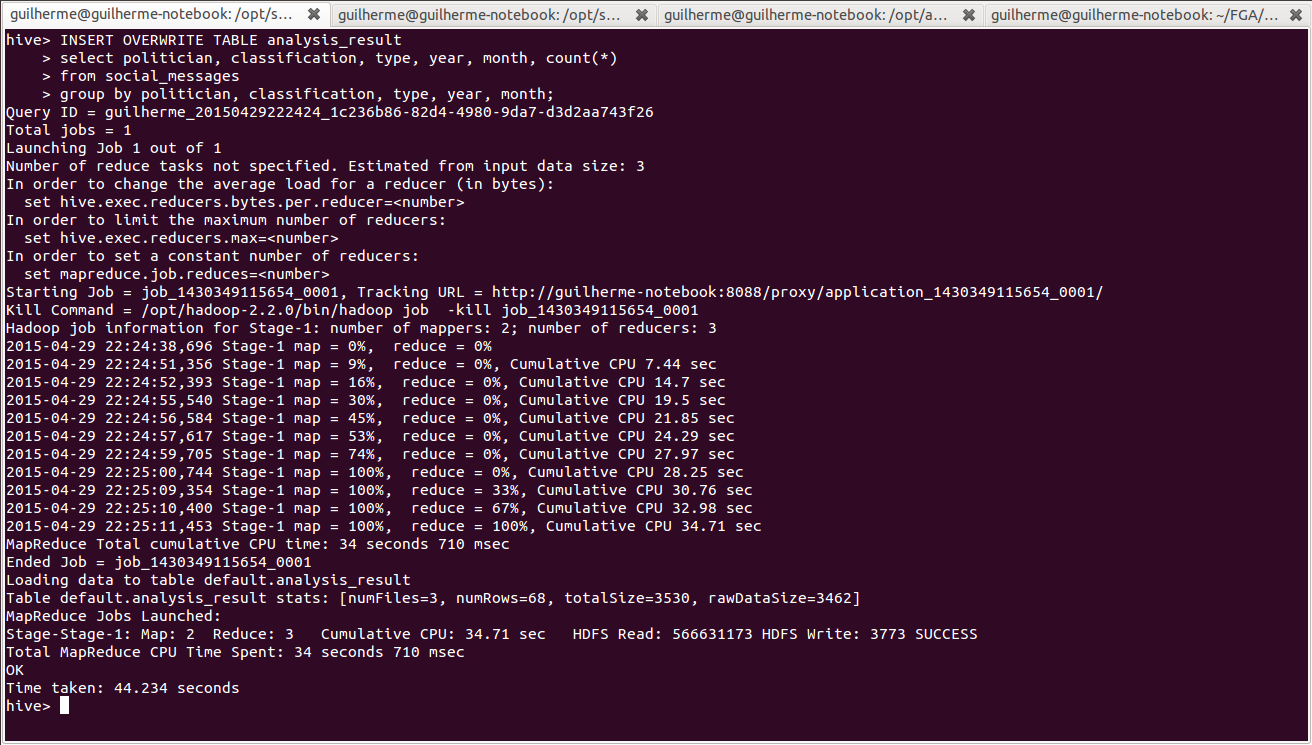
\includegraphics[keepaspectratio=true,scale=0.25]
	  {figuras/job.eps}
	\caption[Tela de execução do comando HiveQL]{Tela de execução do comando HiveQL
	\protect\linebreak Fonte: Autor}
	\label{job-exec}
\end{figure}
\FloatBarrier

Os resultados obtidos após a execução do comando HiveQL foram armazenados na tabela \textit{analysis\_result} e posteriormente transferidos para uma tabela análoga localizada no banco relacional MySQL. A transição entre os dois ambientes, Hive e MySQL, ocorreu com a utilização da ferramenta Sqoop. Os valores desta tabela são exibidos graficamente através da interface \textit{web} construída de acordo com a especificação contida no capítulo \ref{cap:proposta}. Para cada candidato, é possível visualizar a quantidade de mensagens positivas e negativas para os anos de 2014 e 2015. A figura \ref{dilma1} apresenta a página de um dos candidatos analisados.

\begin{figure}[ht!]
	\centering
	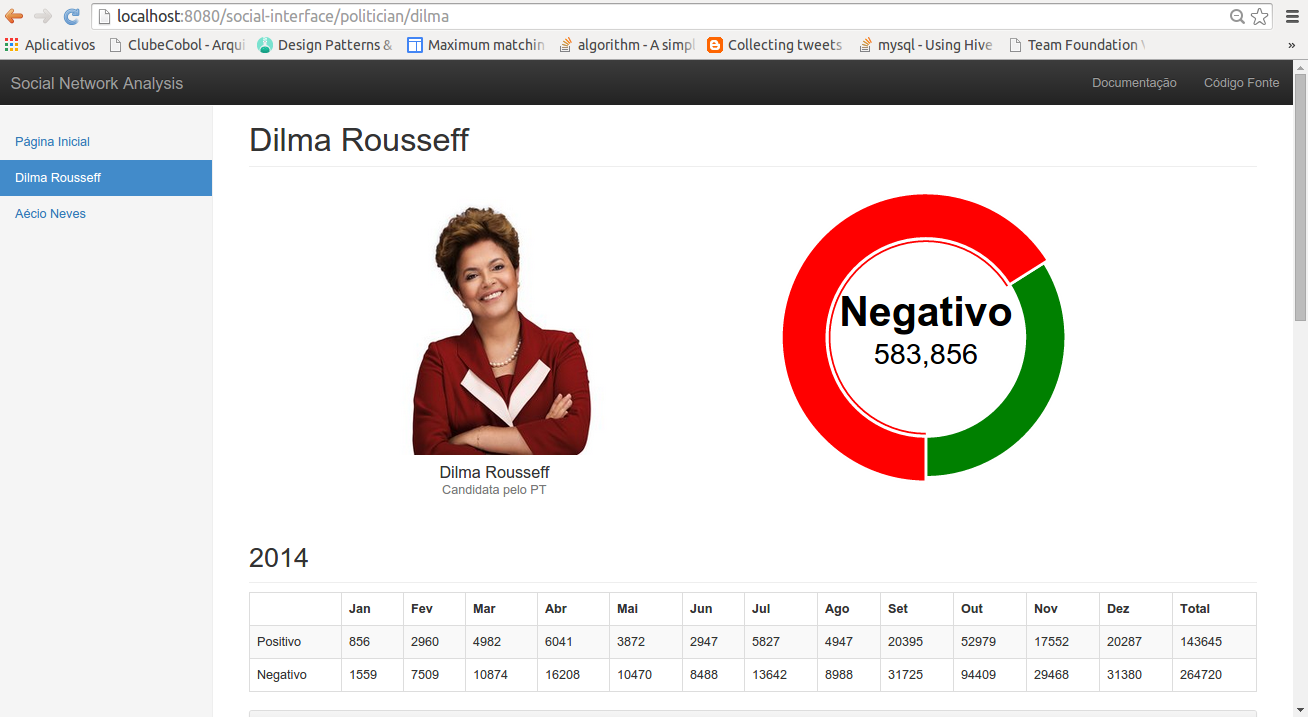
\includegraphics[keepaspectratio=true,scale=0.35]
	  {figuras/dilma1.eps}
	\caption[Tela de resultados para a candidata Dilma Rousseff]{Tela de resultados para a candidata Dilma Rousseff
	\protect\linebreak Fonte: Autor}
	\label{dilma1}
\end{figure}
\FloatBarrier

Cada página de um candidato, além do gráfico com os resultados de todas as mensagens analisadas, também possui, para cada ano, uma tabela com os valores mensais e um gráfico de área ilustrando a análise de sentimentos ao longo dos meses. A figura \ref{dilma1} apresenta o gráfico de área referente ao ano de 2015 para o mesmo candidato mostrado na imagem anterior.

\begin{figure}[ht!]
	\centering
	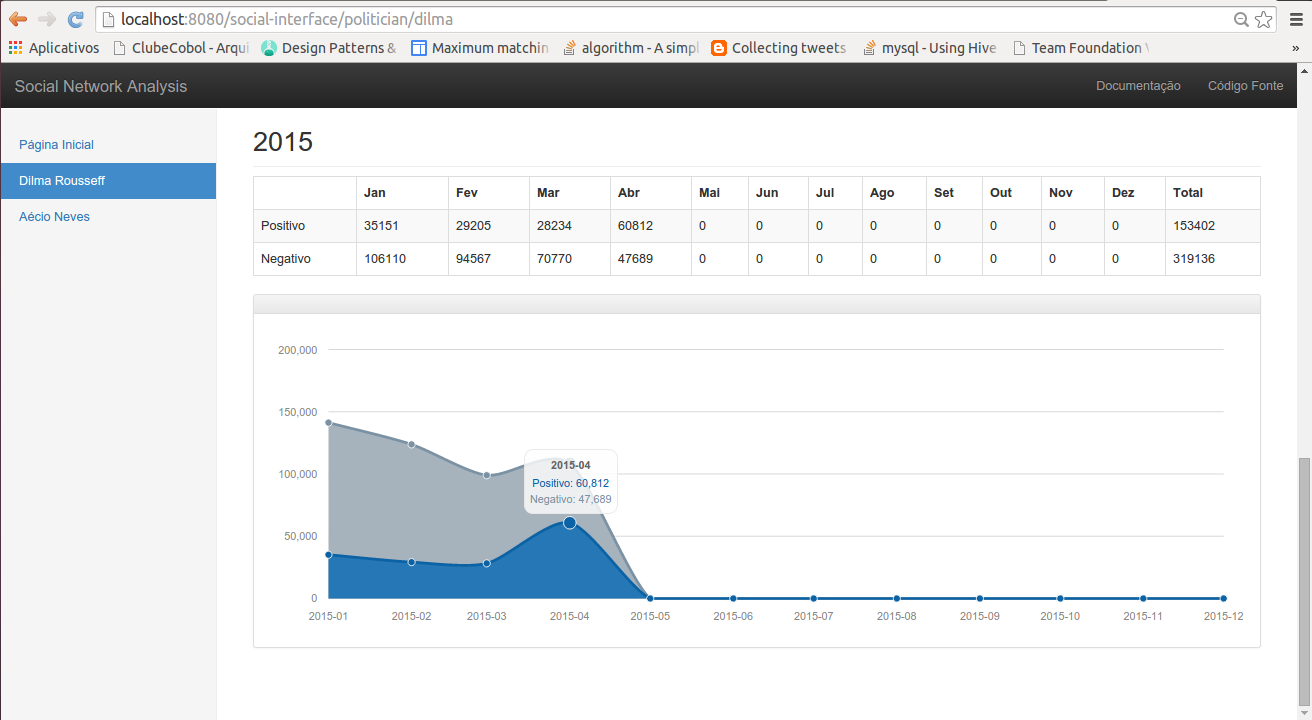
\includegraphics[keepaspectratio=true,scale=0.35]
	  {figuras/dilma2.eps}
	\caption[Gráfico de Área para o ano de 2015]{Gráfico de Área para o ano de 2015
	\protect\linebreak Fonte: Autor}
	\label{dilma2}
\end{figure}
\FloatBarrier

Na figura \ref{aecio}, é ilustrada a página referente a outro candidato analisado, a qual apresenta o mesmo padrão de tela evidenciado na figura \ref{dilma1}.

\begin{figure}[ht!]
	\centering
	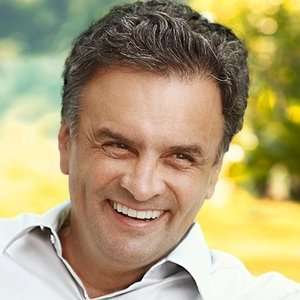
\includegraphics[keepaspectratio=true,scale=0.35]
	  {figuras/aecio.eps}
	\caption[Tela de resultados para o candidato Aécio Neves]{Tela de resultados para o candidato Aécio Neves
	\protect\linebreak Fonte: Autor}
	\label{aecio}
\end{figure}
\FloatBarrier
